\documentclass[handout]{beamer}
\usepackage[utf8]{inputenc}
\usepackage[T2A]{fontenc}
\usepackage[english]{babel}
\usepackage{graphicx}
\usepackage{array}
\usetheme{Warsaw}
\usecolortheme{wolverine}

\usepackage{fontawesome5}
% \usepackage{listings}
\usepackage{listingsutf8}
\usepackage[all]{xy}
\usepackage{changepage}

\definecolor{dkgreen}{rgb}{0,0.6,0}
\definecolor{gray}{rgb}{0.5,0.5,0.5}
\definecolor{mauve}{rgb}{0.58,0,0.82}

\lstdefinelanguage{Haskell}%
  {otherkeywords={},%
   morekeywords={abstype,if,then,else,case,class,data,default,deriving,%
      hiding,if,in,infix,infixl,infixr,import,instance,let,module,%
      newtype,of,qualified,type,where,do,AbsoluteSeek,AppendMode,%
      Array,BlockBuffering,Bool,BufferMode,Char,Complex,Double,Either,%
      FilePath,Float,Int,Word,Integer,Natural,IO,IOError,Ix,LineBuffering,Maybe,%
      Ordering,NoBuffering,ReadMode,ReadWriteMode,ReadS,RelativeSeek,%
      SeekFromEnd,SeekMode,ShowS,StdGen,String,Void,Bounded,Enum,Eq,%
      Eval,ExitCode,exitFailure,exitSuccess,Floating,Fractional,%
      Functor,Handle,HandlePosn,IOMode,Integral,List,Monad,MonadPlus,%
      MonadZero,Num,Numeric,Ord,Random,RandomGen,Ratio,Rational,Read,%
      Real,RealFloat,RealFrac,Show,System,Prelude,EQ,False,GT,Just,%
      Left,LT,Nothing,Right,WriteMode,True,abs,accum,accumArray,%
      accumulate,acos,acosh,all,and,any,ap,appendFile,applyM,%
      approxRational,array,asTypeOf,asin,asinh,assocs,atan,atan2,atanh,%
      bounds,bracket,bracket_,break,catch,catMaybes,ceiling,chr,cis,%
      compare,concat,concatMap,conjugate,const,cos,cosh,curry,cycle,%
      decodeFloat,delete,deleteBy,deleteFirstsBy,denominator,%
      digitToInt,div,divMod,drop,dropWhile,either,elem,elems,elemIndex,%
      elemIndices,encodeFloat,enumFrom,enumFromThen,enumFromThenTo,%
      enumFromTo,error,even,exitFailure,exitWith,fail,%
      filter,filterM,find,findIndex,findIndices,flip,floatDigits,%
      floatRadix,floatRange,floatToDigits,floor,foldl,foldM,foldl1,%
      foldr,foldr1,fromDouble,fromEnum,fromInt,fromInteger,%
      toInteger,fromJust,fromMaybe,fromRat,fromRational,%
      fromRealFrac,fst,gcd,genericLength,genericTake,genericDrop,%
      genericSplitAt,genericIndex,genericReplicate,getArgs,getChar,%
      getContents,getEnv,getLine,getProgName,getStdGen,getStdRandom,%
      group,groupBy,guard,hClose,hFileSize,hFlush,hGetBuffering,%
      hGetChar,hGetContents,hGetLine,hGetPosn,hIsClosed,hIsEOF,hIsOpen,%
      hIsReadable,hIsSeekable,hIsWritable,hLookAhead,hPutChar,hPutStr,%
      hPutStrLn,hPrint,hReady,hSeek,hSetBuffering,hSetPosn,head,%
      hugsIsEOF,hugsHIsEOF,hugsIsSearchErr,hugsIsNameErr,%
      hugsIsWriteErr,id,ioError,imagPart,indices,init,inits,%
      inRange,insert,insertBy,interact,intersect,intersectBy,%
      intersperse,intToDigit,ioeGetErrorString,ioeGetFileName,%
      ioeGetHandle,isAlreadyExistsError,isAlreadyInUseError,isAlpha,%
      isAlphaNum,isAscii,isControl,isDenormalized,isDoesNotExistError,%
      isDigit,isEOF,isEOFError,isFullError,isHexDigit,isIEEE,%
      isIllegalOperation,isInfinite,isJust,isLower,isNaN,%
      isNegativeZero,isNothing,isOctDigit,isPermissionError,isPrefixOf,%
      isPrint,isSpace,isSuffixOf,isUpper,isUserError,iterate,ixmap,%
      join,last,lcm,length,lex,lexDigits,lexLitChar,liftM,liftM2,%
      liftM3,liftM4,liftM5,lines,listArray,listToMaybe,log,logBase,%
      lookup,magnitude,makePolar,map,mapAccumL,mapAccumR,mapAndUnzipM,%
      mapM,mapM_,mapMaybe,max,maxBound,maximum,maximumBy,maybe,%
      maybeToList,min,minBound,minimum,minimumBy,mkPolar,mkStdGen,%
      mplus,mod,msum,mzero,negate,next,newStdGen,not,notElem,nub,nubBy,%
      null,numerator,odd,openFile,or,ord,otherwise,phase,pi,%
      polar,pred,print,product,properFraction,putChar,putStr,putStrLn,%
      quot,quotRem,random,randomIO,randomR,randomRIO,randomRs,randoms,%
      rangeSize,read,readDec,readFile,readFloat,readHex,readInt,readIO,%
      readList,readLitChar,readLn,readParen,readOct,readSigned,reads,%
      readsPrec,realPart,realToFrac,recip,rem,repeat,replicate,return,%
      reverse,round,scaleFloat,scanl,scanl1,scanr,scanr1,seq,sequence,%
      sequence_,setStdGen,show,showChar,showEFloat,showFFloat,%
      showFloat,showGFloat,showInt,showList,showLitChar,showParen,%
      showSigned,showString,shows,showsPrec,significand,signum,sin,%
      sinh,snd,sort,sortBy,span,split,splitAt,sqrt,stderr,stdin,stdout,%
      strict,subtract,succ,sum,system,tail,tails,take,takeWhile,tan,%
      tanh,toEnum,toInt,toInteger,toLower,toRational,toUpper,transpose,%
      truncate,try,uncurry,undefined,unfoldr,union,unionBy,unless,%
      unlines,until,unwords,unzip,unzip3,unzip4,unzip5,unzip6,unzip7,%
      userError,when,words,writeFile,zero,zip,zip3,zip4,zip5,zip6,zip7,%
      zipWith,zipWithM,zipWithM_,zipWith3,zipWith4,zipWith5,zipWith6,%
      zipWith7},%
   sensitive,%
   morecomment=[l]--,%
   morecomment=[n]{\{-}{-\}},%
   morestring=[b]"%
  }[keywords,comments,strings]%

\lstset{
  inputencoding=utf8,
  extendedchars=true,
  language=Haskell,
  showstringspaces=false,
  columns=flexible,
  keepspaces=true,
  basicstyle={\ttfamily},
  numbers=none,
  numberstyle=\tiny\color{gray},
  keywordstyle=\color{blue},
  commentstyle=\color{dkgreen},
  stringstyle=\color{mauve},
  literate={μ}{{$\mu$}}1 {α}{{$\alpha$}}1 {->}{{$\to$}}2 {=>}{{$\Rightarrow$}}2 {<-}{{$\leftarrow$}}2 {≤}{{$\le$}}1
}

\title{All sorts of permutations}
\author[Andrew Lelechenko]{Andrew Lelechenko \\ \texttt{1@dxdy.ru}}
\date{Papers We Love, Kyiv, 22.10.2016}

\begin{document}

\begin{frame}
  \titlepage
\end{frame}

\begin{frame}
\begin{figure}[H]
\centering
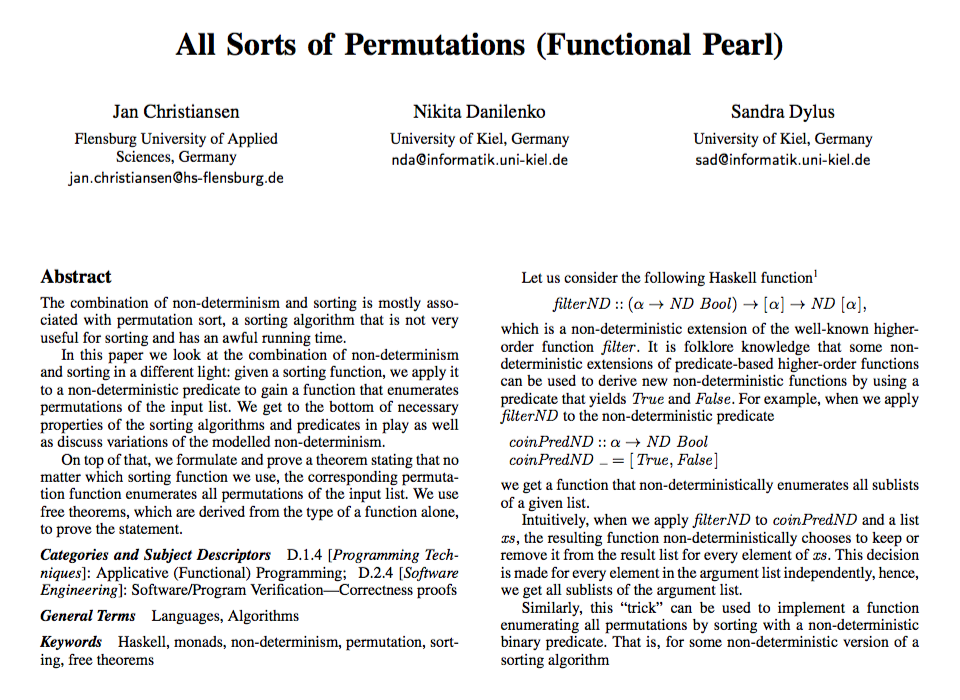
\includegraphics[width=0.9\textwidth]{paper.png}
\end{figure}
\end{frame}

\begin{frame}{Notations}
\begin{itemize}

\item $f :: \alpha \to \beta$ stands for a function, which consumes one argument of type $\alpha$ and returns a value of type $\beta$.

\item $f :: \alpha_1 \to \alpha_2 \to \cdots \to \alpha_n \to \beta$ stands for a function, which consumes $n$ arguments of types $\alpha_1, \alpha_2, \ldots, \alpha_n$ and returns a value of type $\beta$.

\item $[\alpha]$ is a single-linked list of values of type $\alpha$.

\item $[]$ is an empty list.

\item $(a : as)$ is a list with {\em head} $a$ and {\em tail} $as$.

\item $a$, $b$ and $c$ denote single values.

\item $as$, $bs$ and $cs$ denote lists.

\end{itemize}
\end{frame}

\begin{frame}{Deterministic sort}

Typical sort function looks like

\begin{equation*}
\text{sortBy} :: (\alpha \to \alpha \to \text{Bool})
\to [\alpha]
\to [\alpha]
\end{equation*}

E. g.,

\vspace{-4ex}

\begin{align*}
\text{sortBy} ~ (\le) ~ [3,4,1,2] = [1,2,3,4], \\
\text{sortBy} ~ (\ge) ~ [3,4,1,2] = [4,3,2,1].
\end{align*}

Function $(\alpha \to \alpha \to \text{Bool})$ is called a {\em comparator}.

\end{frame}

\begin{frame}{Well-behaved comparators}
\begin{itemize}

\item Consistency: the value of $ a \preceq b $ is always the same.

\item Reflexivity: $a \preceq a$.

\item Antisymmetricity: $a \preceq b$ and $b \preceq a$ iff $a = b$.

\item Transitivity: if $a \preceq b$ and $b \preceq c$, then $a \preceq c$.
\end{itemize}

\bigskip

Otherwise the output of sorting routine:

\begin{itemize}

\item may appear not to be linearly ordered.

\item may appear not to be a permutation of the input.

\end{itemize}

\bigskip

\centerline{\bf What exactly goes wrong, when comparator is ill-behaved?}

\end{frame}

\begin{frame}{Non-deterministic sort}

Let us model a non-deterministic comparator as a function, returning a (maybe empty) list of Bool, representing possible results of comparison. The ultimate example is an {\em uncertain} comparator, which never dares to compare anything:

\begin{align*}
& \text{uncertainCmp} :: \alpha \to \alpha \to [\text{Bool}] \\
& \text{uncertainCmp} ~ a ~ b = [\text{True}, \text{False}]
\end{align*}

The usual {\em certain} comparator looks like

\begin{align*}
& \text{certainCmp} :: \alpha \to \alpha \to [\text{Bool}] \\
& \text{certainCmp} ~ a ~ b = [ a \le b ]
\end{align*}

\end{frame}

\begin{frame}{Sorts and permutations}

Each time, when a non-deterministic comparator returns multiple results, fork execution and combine outputs. Since sorting involves many comparisons, it results in a huge list of possible outcomes.

\begin{itemize}

\item Is each permutation of the input listed? \par
  {\bf Yes,} every sorting algorithm that actually sorts can describe every possible permutation. If there is a permutation that cannot be realised by the sorting algorithm, then there is an input list that cannot be sorted.

\item Is each permutation listed exactly once? \par {\bf It depends.}

\item Is any non-permutation listed? \par {\bf It depends.}
\end{itemize}

Any sorting algorithm may potentially result in a new algorithm for enumerating permutations!

\end{frame}

\begin{frame}[fragile]{Insertion sort --- 1}

\begin{lstlisting}[language=Haskell]
insertSortBy :: forall μ α. Monad μ
             => (α -> α -> μ Bool) -> [α] -> μ [α]
insertSortBy cmp = insertSort
  where
    insertSort :: [α] -> μ [α]
    insertSort []       = return []
    insertSort (a : as) = do
                          bs <- insertSort as
                          insert a bs

    insert :: α -> [α] -> μ [α]
    insert a []       = return [a]
    insert a (b : bs) = do
                        t <- a `cmp` b
                        if t then return (a : b : bs)
                             else (b :) <$> insert a bs
\end{lstlisting}

\end{frame}

\begin{frame}[fragile]{Insertion sort --- 2}

$$\xymatrix@R-2.1pc{
                           &                         & [1,2,3]                &         \\
                           & 1 \le 2 \ar[ur]\ar[ddr] &                        &         \\
                           &                         &                        & [2,1,3] \\
                           &                         & 1 \le 3 \ar[ur]\ar[dr] &         \\
                           &                         &                        & [2,3,1] \\
2 \le 3 \ar[uuuur]\ar[ddr] &                         &                        &         \\
                           &                         & [1,3,2]                &         \\
                           & 1 \le 3 \ar[ur]\ar[ddr] &                        &         \\
                           &                         &                        & [3,1,2] \\
                           &                         & 1 \le 2 \ar[ur]\ar[dr] &         \\
                           &                         &                        & [3,2,1] \\
}$$

\begin{lstlisting}[language=Haskell]
> insertSortBy uncertainCmp [1,2,3]
[[1,2,3],[2,1,3],[2,3,1],[1,3,2],[3,1,2],[3,2,1]]
\end{lstlisting}

\end{frame}

\begin{frame}[fragile]{Selection sort --- 1}

\begin{lstlisting}[language=Haskell]
selectSortBy :: forall μ α. Monad μ
             => (α -> α -> μ Bool) -> [α] -> μ [α]
selectSortBy cmp = selectSort
  where
    selectSort :: [α] -> μ [α]
    selectSort []       = return []
    selectSort (a : as) = do
                          (b, bs) <- selectMin a as
                          (b :) <$> selectSort bs
    selectMin :: α -> [α] -> μ (α, [α])
    selectMin a []       = return (a, [])
    selectMin a (b : bs) = do
                           t <- a `cmp` b
                           let (a', b') = if t then (a, b)
                                               else (b, a)
                           (c, cs) <- selectMin a' bs
                           return (c, b' : cs)
\end{lstlisting}

\end{frame}

\begin{frame}[fragile]{Selection sort --- 2}

\vspace{-4ex}

$$\xymatrix@R-2.2pc{
                             &                          &                        & [1,2,3] \\
                             &                          & 2 \le 3 \ar[ur]\ar[dr] &         \\
                             &                          &                        & [1,3,2] \\
                             & 1 \le 3 \ar[uur]\ar[ddr] &                        &         \\
                             &                          &                        & [3,2,1] \\
                             &                          & 1 \le 2 \ar[ur]\ar[dr] &         \\
                             &                          &                        & [3,1,2] \\
1 \le 2 \ar[uuuur]\ar[ddddr] &                          &                        &         \\
                             &                          &                        & [2,1,3] \\
                             &                          & 1 \le 3 \ar[ur]\ar[dr] &         \\
                             &                          &                        & [2,3,1] \\
                             & 2 \le 3 \ar[uur]\ar[ddr] &                        &         \\
                             &                          &                        & [3,1,2] \\
                             &                          & 1 \le 2 \ar[ur]\ar[dr] &         \\
                             &                          &                        & [3,2,1] \\
}$$

\vspace{-3ex}

\begin{lstlisting}[language=Haskell]
> selectSortBy uncertainCmp [1,2,3]
[[1,2,3],[1,3,2],[3,2,1],[3,1,2],
 [2,1,3],[2,3,1],[3,1,2],[3,2,1]]
\end{lstlisting}

\end{frame}

\begin{frame}[fragile]{Bubble sort --- 1}

\begin{lstlisting}[language=Haskell]
bubbleSortBy :: forall μ α. Monad μ
             => (α -> α -> μ Bool) -> [α] -> μ [α]
bubbleSortBy cmp = bubbleSort
  where
    bubbleSort :: [α] -> μ [α]
    bubbleSort []       = return []
    bubbleSort (a : as) = do
                          (b, bs) <- bubble a as
                          (b :) <$> bubbleSort bs

    bubble :: α -> [α] -> μ (α, [α])
    bubble a []       = return (a, [])
    bubble a (c : cs) = do
                        (b, bs) <- bubble c cs
                        t <- a `cmp` b
                        return $ if t then (a, b : bs)
                                      else (b, a : bs)
\end{lstlisting}

\end{frame}

\begin{frame}[fragile]{Bubble sort --- 2}

\vspace{-4ex}

$$\xymatrix@R-2.2pc{
                             &                          &                        & [1,2,3] \\
                             &                          & 2 \le 3 \ar[ur]\ar[dr] &         \\
                             &                          &                        & [1,3,2] \\
                             & 1 \le 2 \ar[uur]\ar[ddr] &                        &         \\
                             &                          &                        & [2,1,3] \\
                             &                          & 1 \le 3 \ar[ur]\ar[dr] &         \\
                             &                          &                        & [2,3,1] \\
2 \le 3 \ar[uuuur]\ar[ddddr] &                          &                        &         \\
                             &                          &                        & [1,3,2] \\
                             &                          & 3 \le 2 \ar[ur]\ar[dr] &         \\
                             &                          &                        & [1,2,3] \\
                             & 1 \le 3 \ar[uur]\ar[ddr] &                        &         \\
                             &                          &                        & [3,1,2] \\
                             &                          & 1 \le 2 \ar[ur]\ar[dr] &         \\
                             &                          &                        & [3,2,1] \\
}$$

\vspace{-3ex}

\begin{lstlisting}[language=Haskell]
> bubbleSortBy uncertainCmp [1,2,3]
[[1,2,3],[1,3,2],[2,1,3],[2,3,1],
 [1,3,2],[1,2,3],[3,1,2],[3,2,1]]
\end{lstlisting}

\end{frame}

\begin{frame}[fragile]{Quicksort --- 1}

\begin{lstlisting}[language=Haskell]
quickSortBy :: forall μ α. Monad μ
            => (α -> α -> μ Bool) -> [α] -> μ [α]
quickSortBy cmp = quickSort
  where
    quickSort :: [α] -> μ [α]
    quickSort []       = return []
    quickSort (a : as) = do
                     (bs, cs) <- partitionBy (`cmp` a) as
                     xs <- quickSort bs
                     ys <- quickSort cs
                     return $ xs ++ (a : ys)
\end{lstlisting}

\end{frame}

\begin{frame}[fragile]{Quicksort --- 2}

\begin{lstlisting}[language=Haskell]
partitionBy :: Monad μ
            => (α -> μ Bool) -> [α] -> μ ([α], [α])
partitionBy predicate = partition
  where
    partition []       = return ([], [])
    partition (a : as) = do
                         (bs, cs) <- partition as
                         t <- predicate a
                         return $ if t then (a : bs, cs)
                                       else (bs, a : cs)

> quickSortBy uncertainCmp [1,2,3]
[[3,2,1],[2,3,1],[3,1,2],[2,1,3],[1,3,2],[1,2,3]]
\end{lstlisting}

\end{frame}

\begin{frame}[fragile]{Mergesort --- 1}

\begin{lstlisting}[language=Haskell]
mergeSortBy :: forall μ α. Monad μ
            => (α -> α -> μ Bool) -> [α] -> μ [α]
mergeSortBy cmp = mergeSort
  where
    mergeSort :: [α] -> μ [α]
    mergeSort []  = return []
    mergeSort [a] = return [a]
    mergeSort as  = do
                    let l = length as `div` 2
                    let (bs, cs) = splitAt l as
                    xs <- mergeSort bs
                    ys <- mergeSort cs
                    merge xs ys
\end{lstlisting}

\end{frame}

\begin{frame}[fragile]{Mergesort --- 2}

\begin{lstlisting}[language=Haskell]
merge :: [α] -> [α] -> μ [α]
merge as       []       = return as
merge []       bs       = return bs
merge (a : as) (b : bs) = do
                  t <- a `cmp` b
                  if t then (a :) <$> merge as (b : bs)
                       else (b :) <$> merge (a : as) bs

> mergeSortBy uncertainCmp [1,2,3]
[[1,2,3],[2,1,3],[2,3,1],[1,3,2],[3,1,2],[3,2,1]]
\end{lstlisting}

\end{frame}

\begin{frame}{Summary}

\begin{itemize}

\item Insertion sort, quicksort and mergesort enumerates permutations precisely.

\item Selection sort enumerates permutations precisely under assumption of consistency.

\item Bubble sort enumerates permutations precisely under assumption of antisymmericity.

\item Rare algorithms require transitivity for precise enumeration (namely, patience sort by Mallows).

\item Rare algorithms produce not only permutations (namely, two-pass quicksort).

\item Insertion sort, quicksort and mergesort can be transformed into algorithms for enumeration of permutations.

\item But beware to use them as a random permutation generator!

\end{itemize}

\end{frame}

\begin{frame}
\centerline{\Huge\bf Thank you!}
\end{frame}

\end{document}
